% Author: Kimberly Golubeva
% Date: 6 August 2020
% Revised: JMS 28 Feb 2020
% Lauren DeDieu, Jerrod M.~Smith, Kimberly Golubeva and Christian Bagshaw
% A Resource Bank for Writing Intensive Mathematics Courses
% This work is licensed under a  Creative Commons Attribution-NonCommercial-ShareAlike 4.0 International License
% http://creativecommons.org/licenses/by-nc-sa/4.0/
\section{Set Containment}

\begin{xca}{xca:set_containment}
Prove or disprove the following statement. For all sets $A, B$ and $C$,
$$A \cap \left(B \cup C \right) \subseteq \left(A \cap B\right) \cup C\;.$$
\end{xca}

\begin{flaw}{flaw:set_containment} 
This statement is true. From the pictures below, we see that the shaded blue area (top diagram) covered by $A \cap (B \cup C)$ is clearly contained within the shaded orange area (bottom diagram) covered by $(A \cap B) \cup C$.

\def\firstcircle{(0,0) circle (1.5cm)}
\def\secondcircle{(45:2cm) circle (1.5cm)}
\def\thirdcircle{(0:2cm) circle (1.5cm)}


\begin{center}
	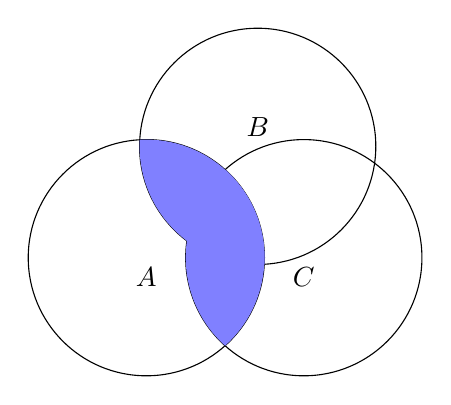
\begin{tikzpicture}
    \draw \firstcircle node[below] {$A$};
    \draw \secondcircle node [above] {$B$};
    \draw \thirdcircle node [below] {$C$};


    \begin{scope}
      \clip \firstcircle;
      \fill[blue!50] \secondcircle;
    \end{scope}


    \begin{scope}
      \clip \firstcircle;
      \clip \secondcircle;
      \fill[blue!50] \thirdcircle;
    \end{scope}
    
    \begin{scope}
      \clip \firstcircle;
      \fill[blue!50] \thirdcircle;
    \end{scope}
    
\end{tikzpicture}%
\end{center}


%%%%%%%%%%%%%%%%%%%%%%%%%%%%%%%%%%%%%%%%%%%%%%%%
\begin{center}
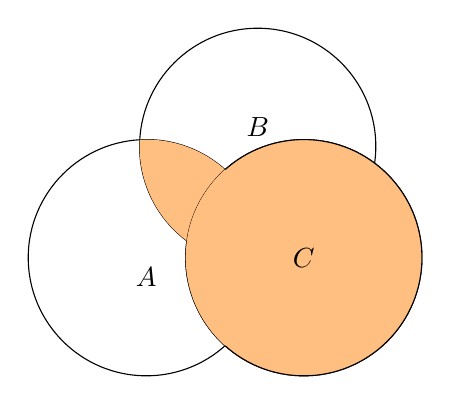
\begin{tikzpicture}
    \draw \firstcircle node[below] {$A$};
    \draw \secondcircle node [above] {$B$};
    \draw \thirdcircle; %node [above] {$C$};

    \begin{scope}
      \clip \firstcircle;
      \fill[orange!50] \secondcircle;
    \end{scope}

    \begin{scope}
      \fill[orange!50] \thirdcircle;
    \draw \thirdcircle node {$C$};
    \end{scope}

    \begin{scope}
      \clip \firstcircle;
      \clip \secondcircle;
      \fill[orange!50] \thirdcircle;
    \end{scope}
    
    \begin{scope}
      \clip \firstcircle;
      \fill[orange!50] \thirdcircle;
    \end{scope}
    
\end{tikzpicture}
\end{center}
\end{flaw}

\clearpage
\subsection{Error classification}

There are several errors
% is only one error ... etc.
 in the Flawed Proof \ref{flaw:set_containment}. 

 
 \begin{description}
 	\item[F-Eg:] Although the logic expressed in the picture is correct, proof by picture is an invalid proof technique. 
 	\item[F-EO:] The entirety of the proof is omitted due to the proof by example error.  
 \end{description}

 
\subsubsection{Error codes}
\begin{itemize}
	\item 	Fundamental Proof by Example (F-Eg)
	\item   Fundamental Error-Caused Omission (F-EO)
\end{itemize}
See Section \ref{sec-error} for more information about error classifications.

\clearpage
\subsection{Corrected proof}

The following is a corrected version of Flawed Proof \ref{flaw:set_containment}. 

\begin{prf}{prf:set_containment} 
Suppose $A, B$ and $C$ are sets. Suppose that $x \in A \cap \left(B \cup C \right).$ Then $x\in A$ and $x \in B \cup C.$ Since $x \in B \cup C,$ we know that $x \in B$ or $x \in C.$ Thus, we have two cases to consider: \\

\noindent \textbf{Case 1:} Suppose that $x \in B$. Then $x \in A$ and $x \in B$, so $x \in A \cap B$. Thus, $x \in \left(A \cap B\right) \cup C.$ \\
\textbf{Case 2:}  Suppose that $x \in C$. Since $x \in C,$ then $x \in \left(A \cap B\right) \cup C.$ \\

\noindent Thus, in both cases $x \in \left(A \cap B\right) \cup C.$ Therefore, We can conclude that $$A \cap \left(B \cup C \right) \subseteq \left(A \cap B\right) \cup C\;.$$
\end{prf}